\documentclass[11pt]{article}
\usepackage[letterpaper,margin=0.78in,headheight=15pt]{geometry}
\usepackage{amsmath,amssymb,amsthm,mathtools,booktabs,array,tabularx,enumitem}
\usepackage[T1]{fontenc}
\usepackage{lmodern,microtype,tikz,fancyhdr,tocloft,hyperref}
\usetikzlibrary{arrows.meta,positioning,calc}
\hypersetup{colorlinks=false,pdfborder={0 0 0},pdftitle={The Sovereign Professor of Professors},pdfauthor={Brian Tenneson; Picard--CIIP-5}}
\pagestyle{fancy}\fancyhf{}\lhead{\small THE SOVEREIGN PROFESSOR OF PROFESSORS}\rhead{\small Research draft 001v2}\cfoot{\thepage}
\setlength{\parindent}{0pt}\setlength{\parskip}{3pt}
\setlength{\cftbeforesecskip}{2pt}\setlist{nosep,leftmargin=*}
\newtheorem{theorem}{Theorem}[section]\newtheorem{proposition}[theorem]{Proposition}\newtheorem{corollary}[theorem]{Corollary}\newtheorem{definition}[theorem]{Definition}\newtheorem{example}[theorem]{Example}\newtheorem{conjecture}[theorem]{Conjecture}
\newcommand{\E}{\mathbb E}\newcommand{\Prob}{\mathbb P}\newcommand{\F}{\mathcal F}\newcommand{\N}{\mathbb N}\newcommand{\Var}{\operatorname{Var}}\newcommand{\one}{\mathbf 1}\newcommand{\spp}{\mathrm{SPP}}
\begin{document}
\begin{center}
{\LARGE\bfseries The Sovereign Professor of Professors\par}\vspace{5pt}
{\large Partial Credit on Logical Objects, Recursive Evaluators,\\ and the Architecture of Mathematical Intelligence\par}\vspace{13pt}
Research Director: Brian Tenneson\\
Mathematical development: Picard--CIIP-5 (ChatGPT research protocol)\\
27 November 2026 $\mid$ Research draft 001v2
\end{center}
\begin{abstract}
We develop the Sovereign Professor of Professors (SPP) as a joint limiting evaluator on three distinct frontiers: partial credit for structured objects with declared correctness judgments, partial credit for evaluators and their recursively defined reports, and assessment of possible changes to the architecture that produces and evaluates those objects. The construction unifies the recursive probabilistic Professor with costed sovereign repair geometry, while preserving the independence of proof verification. A countable, typed, weighted credit ledger gives a common Hilbert-space model of object and meta-level grading; nested authorized evidence yields an exact ignorance-reduction identity. A separate, monotone architectural opportunity coordinate admits a joint almost-sure and mean-square limit as both information and revision allowance increase. We distinguish opportunity from exercised improvement, accuracy from strategic utility, and a limiting estimator from a computable or general mathematical oracle. Counterexamples show why a tower of changing scoring targets, arbitrary evidence-dependent architecture, and greedy grade maximization cannot replace the hypotheses. We supply an exact finite example, a finite-budget decision model, an implementation contract and a settlement register. The main theorems are conditional mathematical results; the full sovereign interpretation and the attainment of general oraclehood remain open.
\end{abstract}
\vspace{2pt}
\textbf{Central thesis.} The SPP is not simply the last Professor in a vertical hierarchy. It is a common limiting assessment of what is correct, how well correctness and progress are assessed, and what lawful changes could improve the capacity to assess or discover it.
{\small\setcounter{tocdepth}{1}\tableofcontents}
\newpage
\section{The three frontiers}
The two parent manuscripts \cite{creative,professor} separate verified mathematical progress from estimated repairability and distinguish improvement of a machine from improvement of the score used to describe it. The present paper takes the Research Director's proposed abstraction seriously: the domain need not consist solely of theorem proofs. It can include any structured logical artifact for which a scoped standard of correctness is meaningful. A Professor's report is itself such an artifact when the grading contract specifies what constitutes a good report. An architectural proposal is another such artifact when the claimed preservation and improvement can be tested against a frozen contract.

The three frontiers are related but not interchangeable. The object frontier concerns candidate proofs, countermodels, formal translations, derivations and related judgments. The evaluator frontier concerns predictions, confidence, estimates of repair cost, and assessments of those reports. The architectural frontier concerns changes to the search, evaluation or control machinery. A fourth operation, settlement, lies outside the credit hierarchy: only a separately authorized checker can certify an object judgment or an admission obligation. A large credit does not constitute settlement.
\begin{figure}[ht]
\centering
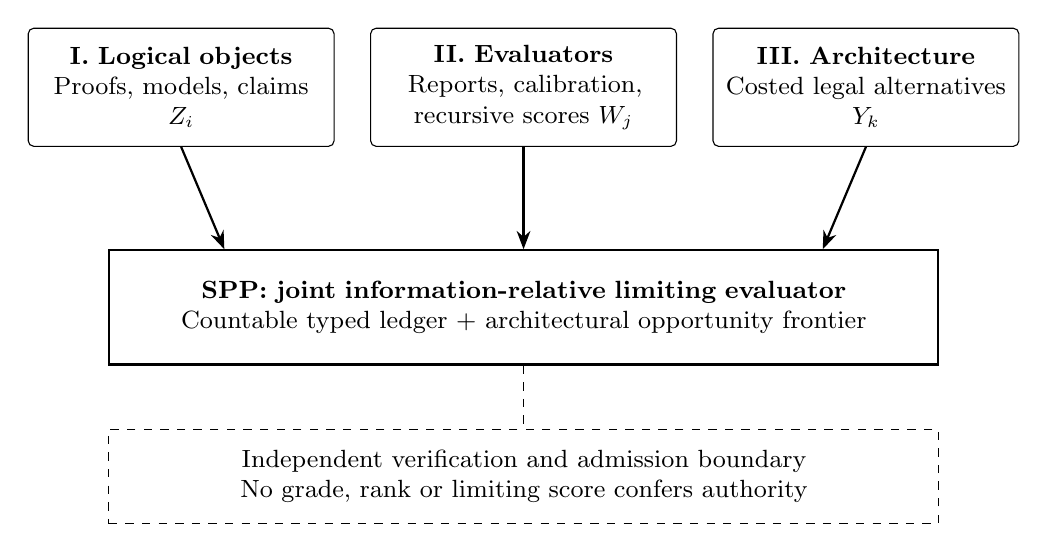
\begin{tikzpicture}[>=Stealth, box/.style={draw,rounded corners=2pt,align=center,minimum height=1.5cm,text width=3.65cm}, every node/.style={font=\small}]
\node[box] (o) {\textbf{I. Logical objects}\\Proofs, models, claims\\$Z_i$};
\node[box,right=0.45cm of o] (m) {\textbf{II. Evaluators}\\Reports, calibration,\\recursive scores $W_j$};
\node[box,right=0.45cm of m] (a) {\textbf{III. Architecture}\\Costed legal alternatives\\$Y_k$};
\node[draw,thick,align=center,minimum height=1.45cm,text width=10.3cm,below=1.3cm of m] (s) {\textbf{SPP: joint information-relative limiting evaluator}\\Countable typed ledger $+$ architectural opportunity frontier};
\draw[->,thick] (o.south)--($(s.north)+(-3.8,0)$);\draw[->,thick] (m.south)--(s.north);\draw[->,thick] (a.south)--($(s.north)+(3.8,0)$);
\node[draw,dashed,align=center,below=0.8cm of s,text width=10.3cm,minimum height=1.2cm] (v) {Independent verification and admission boundary\\No grade, rank or limiting score confers authority};
\draw[dashed] (s)--(v);
\end{tikzpicture}
\caption{The three assessment frontiers. The dashed boundary is deliberately not a fourth score.}
\end{figure}

There are several meanings of ``limit'' in this proposal. A limit of estimates is an epistemic limit; a supremum over legal options is an opportunity limit; a supremum of performance over accessible policies is a capability limit. They may agree in a specially constructed model but need not agree in general. In particular, an eventually constant sequence still has a limit; the term limit point is used in the sense of a limit of a directed family, not a claim that every instance has a nonisolated accumulation point or a unique geometric boundary.

\section{Logical structured information and the correctness boundary}
\begin{definition}[Scoped logical object]
An object is a tuple $x=(\tau,\Gamma,J,a)$ consisting of a type, a context, a declared judgment and an artifact. The contract supplies a semantic predicate $C(x)\in\{0,1\}$ when defined and a certificate checker $V(x,c)\in\{0,1\}$. Soundness means $V(x,c)=1\Rightarrow C(x)=1$. A checker for a refutation certifies the corresponding negative judgment, not the complement of its own acceptance bit.
\end{definition}
The domain may contain judgments of validity, derivability, equivalence, type correctness, or conformance to a formal specification. For a prediction the contract may instead define a realized event and a proper score; for a numerical approximation it may define a tolerance or a bounded loss. Undefined or ill-scoped judgments are excluded or returned as undetermined. Rejection of a certificate is not proof of falsity, and the semantic predicate need not be decidable. This distinction is crucial in incomplete formal systems.

For each eligible object $i$ let $Z_i\in[0,1]$ be a specified grade, not necessarily its correctness indicator. A proof-repair grade can use the parent construction:
\begin{equation} Z_i=\alpha_i q_i+(1-\alpha_i)\exp(-H_i/h_i),\quad h_i>0,\quad 0\leq\alpha_i\leq1,\end{equation}
where $q_i\in[0,1]$ is a normalized relevance-weighted measure of verified capital and $H_i\in[0,+\infty]$ is the infimum of legal repair costs (not necessarily attained). Set $e^{-\infty}=0$. The weights, verifier, target, resource accounting and reference population are frozen for an evaluation episode. A separate coordinate $C_i$ can encode semantic correctness if it is well defined and measurable. Another can encode existence of a checked certificate by a budget deadline. Neither of these coordinates is in general equal to the repair grade.

\begin{proposition}[No scalar settlement implication]
Without additional restrictions on the grading contract, $Z_i=1$ does not imply that the artifact has a certificate or that its declared judgment is correct.
\end{proposition}
\begin{proof}Take $\alpha_i=1$ and let the declared judgment be the false statement $0=1$ in standard arithmetic, with no accepting certificate under a sound checker. A normalized capital ledger that awards full credit for a verified prerequisite (for example $0=0$) gives $q_i=1$ and hence $Z_i=1$, even with $H_i=+\infty$. Such a ledger is permitted because no assumption links full capital to the truth of the target. Separately, when $\alpha_i=0$, a nonterminal state with a zero-cost legal path to a checked goal has $H_i=0$ and grade one without current acceptance.\end{proof}

Thus partial credit is a valuation on the boundary between incomplete evidence and certified resolution. It can orient search without changing the truth condition. The distinction generalizes naturally to a Professor's report: an exact prediction of a score, for instance, need not be an exact proof of the original statement.

\section{Credit on Professors: a typed recursive ledger}
Work on a common probability space $(\Omega,\mathcal A,\Prob)$ and let $\F_0\subseteq\F_1\subseteq\cdots$ be the cumulative authorized evidence, with $\F_\infty=\sigma(\bigcup_n\F_n)$. Each target is a bounded measurable random variable. The law may describe hidden instances or experimental outcomes; it is not validated by the fact that several agents agree.

\begin{definition}[Frozen report and meta-target]
For a target $Z_i$ and an actual report $r_{i,t}\in[0,1]$ measurable in $\F_t$, archive the report together with its target ID, contract and observation cutoff. Its realized quadratic quality is
\begin{equation}W_{i,t}=1-(Z_i-r_{i,t})^2.\end{equation}
At a subsequent review $n\geq t$, the ideal meta-credit is $G_{i,t;n}=\E[W_{i,t}\mid\F_n]$. If a report $g\in[0,1]$, measurable at its declared review cutoff, estimates this meta-target, it may itself be frozen and graded by $1-(W_{i,t}-g)^2$. A new target is created rather than overwriting a previous one.
\end{definition}
For $P_{i,n}=\E[Z_i\mid\F_n]$ and $V_{i,n}=\Var(Z_i\mid\F_n)$,
\begin{equation}1-G_{i,t;n}=V_{i,n}+(P_{i,n}-r_{i,t})^2.\label{eq:meta}\end{equation}
Indeed, the residual $Z_i-P_{i,n}$ has conditional mean zero. This exact identity inherited from \cite{professor} distinguishes residual uncertainty from disagreement with the frozen answer. A forecast that differs from the realized target can still receive high quadratic credit; one realized score does not establish calibration.

\begin{definition}[Typed ledger]
Choose a countable registry $\mathcal J$ of object and recursive report targets $X_j\in[0,1]$. Each report target points to an earlier frozen target and report. Require that each node has a finite chain of ancestors ending at an object target; in particular, the dependency graph has no cycles or infinite regress. Choose strictly positive weights $w_j$ with $\sum_{j\in\mathcal J}w_j=1$. Define $\mathcal H=\ell^2(\mathcal J,w)$ and the ledger $X=(X_j)_j$. For a finite nonempty registry use any strictly positive normalized weights and interpret every truncation beyond its size as the full registry.
\end{definition}
The full registry is a mathematical evaluation design, not a claim that an online agent already possesses future reports. Potential future report coordinates may be defined in advance as measurable random variables by a fixed protocol; their scoring is retrospective and cannot authorize disclosure before creation. Alternatively apply the theorem to an already frozen archive and extend the archive in successive evaluation episodes. The theorem does not cover arbitrary retroactive changes of targets or weights.

At every level the Professor retains its estimates of original objects, not just the newest score of a score. To see why, take a deterministic $X_0=1$ and a chain of reports $r_d=0$; define $X_{d+1}=1-(X_d-r_d)^2$. Then $X_d$ alternates $1,0,1,0,\ldots$. Even perfect access to each realized target does not make this moving-target sequence converge. A limit of the entire ledger is a different construction.

\begin{figure}[ht]
\centering
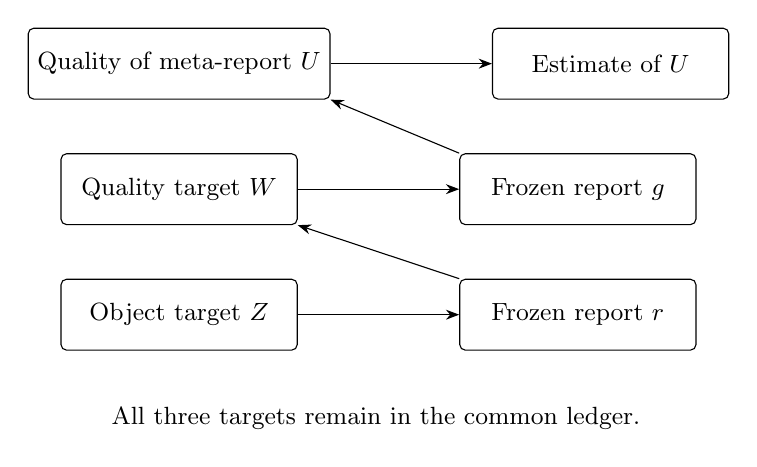
\begin{tikzpicture}[>=Stealth,every node/.style={font=\small},b/.style={draw,rounded corners=2pt,minimum width=3cm,minimum height=0.9cm,align=center}]
\node[b] (x) {Object target $Z$};
\node[b,above=0.68cm of x] (w) {Quality target $W$};
\node[b,above=0.68cm of w] (u) {Quality of meta-report $U$};
\node[b,right=2.05cm of x] (p) {Frozen report $r$};
\node[b,right=2.05cm of w] (g) {Frozen report $g$};
\node[b,right=2.05cm of u] (l) {Estimate of $U$};
\draw[->] (x)--(p);\draw[->] (w)--(g);\draw[->] (u)--(l);
\draw[->] (p.north west)--(w.south east);\draw[->] (g.north west)--(u.south east);
\node[align=center,below=0.6cm of x,xshift=2.5cm] {All three targets remain in the common ledger.};
\end{tikzpicture}
\caption{Recursive credit produces new, separately typed objects. It never replaces the original grading question.}
\end{figure}

\section{A joint ignorance theorem for logical and recursive credit}
Define $M_n=(\E[X_j\mid\F_n])_j$ and $I_n=\E\|X-M_n\|_{\mathcal H}^2$. All components are simultaneously defined after discarding a single null set. The nonnegative summable weights give finite expected risk, regardless of the number of meta-levels.
\begin{theorem}[Typed Professor limit]\label{thm:ledger}
For the frozen registry and nested evidence,
\begin{align}M_n&\longrightarrow M_\infty=(\E[X_j\mid\F_\infty])_j\quad\text{a.s. in }\mathcal H\text{ and in }L^2(\Omega;\mathcal H),\\
I_n-I_{n+1}&=\E\|M_{n+1}-M_n\|_{\mathcal H}^2\geq0.\label{eq:ignorance}\end{align}
The limiting estimator uniquely minimizes weighted squared risk among $\F_\infty$-measurable square-integrable ledger reports, up to almost-sure equality. Exact simultaneous recovery occurs iff every $X_j$ has an $\F_\infty$-measurable version.
\end{theorem}
\begin{proof}For each $j$, bounded martingale convergence and L\'evy's upward theorem \cite{williams} give almost-sure and $L^2$ convergence. Countability supplies one probability-one event. On that event the squared norm of the difference is a weighted sum of terms bounded by one. Dominated convergence over $j$ gives norm convergence, and bounded convergence over $\Omega$ gives $L^2$. Coordinatewise conditional orthogonality gives the risk decrement; Tonelli permits summation. For any measurable competitor $R$, orthogonality yields
\[\E\|X-R\|^2=\E\|X-M_\infty\|^2+\E\|R-M_\infty\|^2.\]
Strictly positive weights imply zero risk iff every coordinate has zero risk, which is equivalent to measurability in the limiting evidence.\end{proof}

\begin{corollary}[Finite registry truncation and practical error]
If only coordinates $1,\ldots,m$ are reported and the others are filled with zero, the truncation contributes at most $\sum_{j>m}w_j$ to expected squared distance from the ideal full report. For any actual $\F_n$-measurable ledger report $R_n\in[0,1]^{\mathcal J}$,
\[\E\|X-R_n\|^2=I_n+\E\|R_n-M_n\|^2.\]
Consequently $R_n\to M_\infty$ in mean square if its excess risk tends to zero. If the excess risks are summable, convergence also holds almost surely.
\end{corollary}
\begin{proof}The tail bound follows from the coordinate bound one. The risk identity is the same orthogonal decomposition at $\F_n$. Use the triangle inequality for mean-square convergence and Markov's inequality plus Borel--Cantelli for almost-sure convergence.\end{proof}

This theorem is a common mathematical limit across all fixed logical and meta-logical targets. The word ``all'' is restricted to the declared registry. One cannot infer uniform accuracy over an unweighted infinite collection from weighted convergence; at a given stage a low-weight coordinate can be badly estimated while contributing little to total ignorance. Each fixed positive-weight coordinate nevertheless converges to its own limiting posterior; irreducible target error may persist. More generally, finite practical grading accuracy must be demonstrated, not inferred from the existence of the ideal hierarchy.
\section{Meta partial credit on architecture}
Let $s$ be a complete operational state, including the implementation, verified BANK, history, resource ledger and permissions. Hold fixed the object judgment, checker, score calibration and comparison protocol. An ordinary transition changes the state without a sovereign commit; a revision edge represents the legal execution of an admitted change in the declared operational contract. The graph contains possible executions, not a claim that those executions have occurred in the actual history. All edges have nonnegative charged costs. Costs include proposal, checking, migration and execution. A proposed gift that is rejected or undetermined is not a revision edge; its incurred costs remain chargeable.

For a fixed initial state and goal set $G$, define the costed horizon
\begin{equation}H_k(s)=\inf\{\mathrm{cost}(\pi):s\leadsto G,\ r(\pi)\leq k\},\qquad k\in\N_0,\end{equation}
with empty infimum $+\infty$ and $r$ counting commits, not atoms. In finite graphs it can be computed by shortest paths in the lifted state graph $(s,k)$, with a gift decrementing $k$. This is the architectural construction of \cite{creative}. The feasible sets grow with $k$, so $H_{k+1}\leq H_k$. For a common $q\in[0,1]$, $\alpha\in[0,1]$ and $h>0$ independent of the allowance $k$, set
\[Y_k=\alpha q+(1-\alpha)e^{-H_k/h},\qquad A_k=Y_k-Y_0.\]
Here $A_k$ is the sovereign opportunity credit. It represents an advantage in the feasible envelope, not an observed architectural improvement. It is nonnegative because retaining the ordinary path is permitted. For stochastic worlds assume $q$ and the $H_k$ are measurable; a fixed countable vertex and edge universe with measurable availability, costs, initial state and goal membership is one sufficient setting (take the infimum over countably many finite paths). For adversarial games a specified strategy value, rather than an existential shortest path, is needed.

\begin{definition}[Three architectural credit records]
A proposed intervention receives three separate records: (i) admission evidence and unresolved obligations; (ii) predicted incremental utility against a named baseline; (iii) realized or certified post-intervention change against the same baseline. The third is absent until execution or an explicitly scoped certificate establishing the claimed comparison. A favorable forecast is neither admission nor execution.
\end{definition}

\begin{proposition}[Robust comparison of intervention grades]
Suppose independently justified intervals satisfy $q^-\leq q\leq q^+$ and $L\leq H\leq U$, with corresponding primed intervals after revision. Define $B^- =\alpha q^-+(1-\alpha)e^{-U/h}$ and $B^+=\alpha q^++(1-\alpha)e^{-L/h}$. If $B^{\prime-}>B^+$, the successor grade strictly exceeds the parent grade on every permitted realization. If the sole constraints are closed grade intervals whose Cartesian product is allowed, strict separation is necessary for such an interval-only guarantee. Additional dependencies between the two grades can permit a stronger conclusion.
\end{proposition}
\begin{proof}The exponential is decreasing in the horizon. The first conclusion follows by chaining the bounds. For necessity select the smallest allowed successor grade and largest allowed parent grade.\end{proof}
This comparison requires bounds valid in the revised graph; a lower horizon bound can become invalid when a shortcut is introduced. It also does not by itself certify the intervention's cost-effectiveness. In particular, compare total budgets including any migration overhead rather than comparing two machines after giving one free setup.

\section{The Sovereign Professor as a common limit}
For each architecture allowance $k$ define $P_{n,k}=\E[Y_k\mid\F_n]$. The index $n$ measures authorized information, not physical clock time. Assume the same nested aggregate filtration and common probability law for every $k$. In particular, the counterfactual opportunity target is defined even when the actual evaluator does not exercise a gift. A later section handles actual evolution separately.
\begin{theorem}[Joint frontier convergence]\label{thm:joint}
Let $0\leq Y_0\leq Y_1\leq\cdots\leq1$ be measurable and $Y_\infty=\sup_kY_k$. Then the following hold:
\begin{align}
P_{n,k+1}&\geq P_{n,k}\quad\text{a.s.},\\
\lim_{n,k\to\infty}P_{n,k}&=P_{\infty,\infty}:=\E[Y_\infty\mid\F_\infty]\quad\text{a.s. and in }L^2.\label{eq:joint}
\end{align}
Here the joint limit means convergence for all $n,k$ simultaneously sufficiently large, not just along a selected diagonal. Both iterated limits agree with it. For fixed $k$, the risk $\E[(Y_k-P_{n,k})^2]$ decreases with $n$ by the expected squared revision.
\end{theorem}
\begin{proof}Order preservation gives the first claim. Choose simultaneous versions of the conditional expectations for all finite $n,k$, $P_{n,\infty}$ and $P_{\infty,k}$ on a common probability-one event. For each fixed $K$ and all $k\geq K$,
\[P_{n,K}\leq P_{n,k}\leq P_{n,\infty}.\]
By L\'evy's upward theorem the outer terms converge as $n\to\infty$ to $\E[Y_K\mid\F_\infty]$ and $P_{\infty,\infty}$. Conditional monotone convergence gives $\E[Y_K\mid\F_\infty]\uparrow P_{\infty,\infty}$ as $K\to\infty$. Given any positive tolerance on the common event, choose $K$ to make the limiting lower bound close and then choose $n$ large for both outer bounds. This establishes joint almost-sure convergence. Bounded convergence along any sequence of index pairs tending to infinity gives the joint $L^2$ limit (otherwise a violating sequence could be selected). Conditional monotone convergence for fixed $n$ and martingale convergence for fixed $k$ give both iterated limits. The risk statement is scalar conditional orthogonality.\end{proof}

\begin{figure}[ht]
\centering
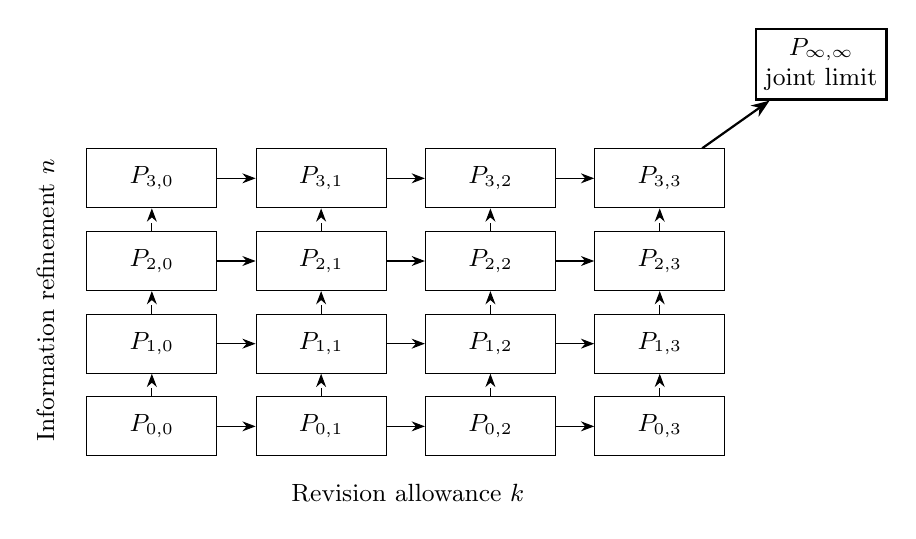
\begin{tikzpicture}[>=Stealth,every node/.style={font=\small}]
\foreach \n in {0,1,2,3}{\foreach \k in {0,1,2,3}{\node[draw,minimum width=1.65cm,minimum height=0.75cm] (p\n\k) at (2.15*\k,1.05*\n) {$P_{\n,\k}$};}}
\foreach \n in {0,1,2,3}{\foreach \k in {0,1,2}{\pgfmathtruncatemacro{\j}{\k+1}\draw[->] (p\n\k)--(p\n\j);}}
\foreach \n in {0,1,2}{\foreach \k in {0,1,2,3}{\pgfmathtruncatemacro{\j}{\n+1}\draw[->,dashed] (p\n\k)--(p\j\k);}}
\node[draw,thick,align=center] (lim) at (8.5,4.6) {$P_{\infty,\infty}$\\joint limit};
\draw[->,thick] (p33)--(lim);
\node[rotate=90] at (-1.35,1.6) {Information refinement $n$};
\node at (3.25,-0.85) {Revision allowance $k$};
\end{tikzpicture}
\caption{Horizontal arrows are ordered credit improvements. Vertical arrows reduce expected estimation error but need not increase the reported score.}
\end{figure}

To unite this with the ledger, let $T_m$ retain the first $m$ fixed targets and fill the remainder with zero. Define
\[S_{n,m,k}=(T_m M_n, P_{n,k}, P_{n,k}-P_{n,0})\in\mathcal H\oplus\mathbb R^2.\]
\begin{corollary}[SPP common limit]\label{cor:spp}
Under Theorems \ref{thm:ledger} and \ref{thm:joint},
\begin{equation}\boxed{S_{n,m,k}\longrightarrow \spp_\infty=(M_\infty,P_{\infty,\infty},P_{\infty,\infty}-P_{\infty,0})}\end{equation}
as $n,m,k\to\infty$ jointly, almost surely and in mean square. All six orders of iterated limits exist and agree.
\end{corollary}
\begin{proof}The ledger error is bounded by $\|M_n-M_\infty\|+(\sum_{j>m}w_j)^{1/2}$. The other coordinates converge by Theorem \ref{thm:joint} and the fixed-$k=0$ martingale limit. The estimates are bounded, so the same sequential argument establishes mean-square convergence. For iterated limits, $m$ acts only on the ledger and truncations converge uniformly in $n$; the $n,k$ iterates of the other coordinates agree by Theorem \ref{thm:joint}.\end{proof}
The index $m$ is breadth of the declared typed registry; a suitable enumeration exhausts every finite recursive depth but $m$ is not itself a count of physical Professors. The result supplies a rigorous version of a common limit at multiple partial-credit boundaries. No assumption of independence between targets or between their errors is needed. No universal rate, finite attainment or physical implementation is inferred.
\section{What the boundary means, and what it cannot mean}
\subsection{Information, opportunity, and capability are separate}
The risk $I_n$ is monotone in information; opportunity $Y_k$ is monotone in allowance. It does not follow that risk decreases with $k$ since its target changes. For example, with no evidence and a fair Bernoulli variable $B$, take $Y_0=0$ and $Y_1=B$. Opportunity increases and risk rises from zero to $1/4$. Conversely, a larger allowance can make a grade constant and easier to predict. Nor is any realized $P_{n,k}$ monotone in $n$.

For a frozen workload and a fixed budget $T$, let $\Pi_k(T)$ be the nonempty sets of feasible policies with at most $k$ commits and let $U(\pi)\in[0,1]$ be their common-law expected outcome utility (e.g., verified settlement by deadline). If the policies are nested, then
\[C_k(T)=\sup_{\pi\in\Pi_k(T)}U(\pi)\uparrow C_\infty(T)=\sup_k C_k(T).\]
This is a third limit, of capability. An actual policy need not attain the supremum, and existence of a path does not imply that an agent can discover it on budget. In general $C_k(T)$ is not $Y_k$: a cheap path may be very difficult to locate. Moreover a bounded risk target may not identify which policy has the largest utility.

\begin{proposition}[When ignorance controls capability regret]\label{prop:regret}
For a nonempty finite action set $D$ with a fixed measurable tie-breaking rule, let $u_a=\E[U_a\mid\F]$ be the expected common-contract utility of each feasible action. Suppose an $\F$-measurable approximate vector $\hat u_a$ is used to choose $\hat a\in\arg\max_a\hat u_a$. Then
\[\max_a u_a-u_{\hat a}\leq 2\max_a|u_a-\hat u_a|.\]
If all action coordinates have positive weights $w_a$ with minimum $w_*>0$, the expected regret is at most $2(\E\sum_a w_a|u_a-\hat u_a|^2/w_*)^{1/2}$.
\end{proposition}
\begin{proof}If $a^*$ maximizes $u_a$, then $u_{a^*}-u_{\hat a}\leq |u_{a^*}-\hat u_{a^*}|+|\hat u_{\hat a}-u_{\hat a}|$ by the choice of $\hat a$. Bound the maximum coordinate error by the weighted norm divided by $\sqrt{w_*}$ and apply Cauchy--Schwarz.\end{proof}
\begin{theorem}[Growing decision frontiers]\label{thm:growing}
Let $D_1\subseteq D_2\subseteq\cdots$ be nonempty finite deterministic action sets, and let $u_a\in[0,1]$ be the conditional expected utility of action $a$ given a fixed comparison information set $\mathcal G$. Write $C_m=\max_{a\in D_m}u_a$ and $C_*=\sup_{a\in\cup_m D_m}u_a$. Suppose $\hat u_{m,a}$ are $\mathcal G$-measurable estimates and choose $\hat a_m$ maximizing them over $D_m$ by a fixed deterministic tie-breaking rule. If
\[\E\sum_{a\in D_m}|u_a-\hat u_{m,a}|^2\longrightarrow0,\]
then $\E[C_*-u_{\hat a_m}]\to0$. A sufficient condition for the premise, for positive weights $w_a$ and weighted error $e_m^2=\E\sum_{a\in D_m}w_a|u_a-\hat u_{m,a}|^2$, is $e_m^2/\min_{a\in D_m}w_a\to0$.
\end{theorem}
\begin{proof}The nonnegative difference splits as $C_*-C_m+C_m-u_{\hat a_m}$. The expected first term vanishes by bounded monotone convergence. The expected second term is bounded by twice the square root of the displayed sum in expectation, by Proposition \ref{prop:regret} and Cauchy--Schwarz. The sufficient condition follows by comparing weighted and unweighted sums.\end{proof}
This is an explicit sufficient condition for capability convergence within the accessible decision frontier. It makes no assertion that the frontier exhausts the capabilities of an oracle, that the estimates can be obtained effectively, or that the required resource schedule exists.

Thus learning the correct targets can improve decision quality, provided they cover the feasible actions and the controller actually uses them. For a countable action family one can approximate the supremum by finite sets, but needs a coverage or tail-regret argument. Weighted mean-square convergence alone cannot control the maximum over a growing number of tiny-weight action coordinates.

\subsection{Failure of the common-limit hypotheses}
The common filtration assumption is substantive. If revision allowance changes what a Professor may observe, a single $\F_n$ may not describe the experiment. A simple double array $b_{n,k}=\one_{\{n\geq k\}}$ has one iterated limit equal to one and the other equal to zero. It cannot arise under Theorem \ref{thm:joint}, since it is decreasing rather than increasing in $k$. It can describe a practical report that defaults to zero until disclosure. Even exact conditional estimates can fail with allowance-dependent information: let $B$ be a fair bit, set $Y_k=B$ for every $k$, and let $\F_{n,k}$ be trivial for $n<k$ and $\sigma(B)$ otherwise. Each fixed-$k$ filtration is nested, but the posterior is $1/2$ for $n<k$ and $B$ otherwise. The $n$-first iterated limit is $B$ and the $k$-first limit is $1/2$, which disagree almost surely. New convergence claims require explicit compatibility of the information and opportunity systems.

Likewise the topological or Pareto interpretation of the SPP must be declared. A natural attainable set is the closure of tuples of risk, utility and cost under a fixed experiment. There may be many nondominated points and no single point achieving the best value in every coordinate. For example two feasible policies with (risk,utility,cost) equal to $(0.1,0.4,1)$ and $(0.2,0.9,1)$ are incomparable when low risk and high utility are preferred. The canonical posterior limit is not automatically a Pareto-optimal implementable system. It is a reference boundary against which such systems can be compared.

\section{Actual evolution: the Professor as student and architect}
The SPP is an evaluator; an operational SPP controller may also propose revisions. If the underlying state changes with time, write $Z_t$ for the grade under the same frozen rubric of the evolving state, and $p_t=\E[Z_t\mid\F_t]$. Then
\begin{theorem}[Moving-target drift]\label{thm:drift}
For uniformly bounded measurable $Z_t$ (in particular, $0\leq Z_t\leq1$) and nested $\F_t$,
\[\E[p_{t+1}\mid\F_t]-p_t=\E[Z_{t+1}-Z_t\mid\F_t].\]
If the right side is nonnegative almost surely for every $t$, $p_t$ is a bounded submartingale and converges almost surely and in $L^2$. A fixed target gives the usual martingale. Neither conclusion forces actual states or architectures to stabilize.
\end{theorem}
\begin{proof}Apply the tower property to $p_{t+1}$. Under the nonnegative drift condition use bounded submartingale convergence and bounded convergence for the squared error.\end{proof}
For example a state can alternate between two distinct implementations with identical grades. If a system can change the grading parameters instead of its capability, it can artificially increase credit: for fixed positive finite $H$, $e^{-H/h}$ strictly increases with $h$. The assessment contract must therefore be separated from the architecture being changed. A revision to the assessment contract is a new experiment with an explicitly justified comparison map, not an in-place improvement claim.

\subsection{Information acquisition versus architectural investment}
Fix a budget and an objective. The decision to purchase a review depends on its expected reduction in risk, while a decision to buy a revision depends on expected benefit under the new policy envelope and all costs. For a common fixed target vector $X$ and a proposed experiment revealing $\F'\supseteq\F$, let $M=\E[X\mid\F]$ and $M'=\E[X\mid\F']$. The one-step expected reduction in conditional weighted squared risk is
\[D=\E[\|M'-M\|^2\mid\F].\]
This follows by conditional orthogonality. If a review costs $c$ in a declared unit, and risk reduction is the only benefit, purchase is strictly preferred to stopping exactly when $D>\lambda c$, for conversion factor $\lambda>0$. The result does not cover an experiment that also changes the target or consumes resources needed for proof search.

For a finite-horizon controlled model let $b$ be a sufficient information state (e.g., a belief and operational state), $t$ the remaining integer resource budget, and $a$ an admissible action with charged integer cost $c(a)\geq1$. Let $J(b)$ be the best terminal expected utility, with the terminal options including stopping, reporting and accepting only checked certificates where applicable. Write $K(db'\mid b,a)$ for the state transition law. Then
\begin{equation}V(b,t)=\max\left\{J(b),\max_{a:c(a)\leq t}\int V(b',t-c(a))K(db'\mid b,a)\right\}.\label{eq:bellman}\end{equation}
The maximum is over admissible actions at $b$ with $c(a)\leq t$; if none exist, set $V(b,t)=J(b)$ (in particular $V(b,0)=J(b)$). For finite state and action sets with the stated Markov sufficiency, the recursion is exact by induction on $t$: every first action spends positive resources and leads to a strictly smaller problem. One may choose a weighted terminal objective combining verified success, predictive loss and novelty, but those weights are a decision-design choice, not a mathematical definition of truth. Costs already charged against the budget need not be counted again unless the terminal objective intentionally penalizes cost as well.

\begin{example}[Why perfect grading does not imply good strategy]
Let $\alpha=1/2$, $h=1$, and $q(s)=1$. An ordinary route reaches a familiar proof at cost four. A detour of cost one reaches $p$ with $q(p)=0$ and no ordinary settlement path; the only goal-reaching routes from $s$ are the two described here. An admitted revision of cost one followed by an ordinary step of cost one reaches a novel proof. With one commit allowed, the grade at $s$ is $(1+e^{-3})/2$, but at $p$ it is $e^{-2}/2$. A controller accepting only nondecreasing grades rejects the first step of the cheaper, novel route. Both grades are exact. This instantiates the greedy barrier in \cite{creative}; a finite-budget controller can instead compare terminal outcomes under the complete costed route.\end{example}
The strategic Professor grades not only the last report but also the decision rule which uses it. A policy report may itself be scored retrospectively against a predeclared regret or utility target and entered in the same typed ledger. This is a precise sense in which meta partial credit can reach actual architecture without confusing a prediction with its execution.
\section{An exact finite experiment}
Consider two independent fair bits $X$ and $B$. The bit $X$ is a hidden correctness judgment. The bit $B$ states whether a charged revision route is available; its availability is assumed to have been admitted in the abstract graph when $B=1$. The ordinary horizon is four in both worlds. One gift may reduce the total charged horizon to two if $B=1$, otherwise it remains four. Set $\alpha=0$, $h=1/\log 2$. Therefore $Y_0=1/16$ and $Y_1=1/16+3B/16$.

Professor 0 has no evidence and reports $r=1/2$ for $X$. Professor 1 receives a binary signal $L$ through a symmetric channel: $\Prob(L=x\mid X=x)=3/4$ for each $x\in\{0,1\}$, with $L$ independent of $B$ conditional on $X$. Professor 2 learns $B$. Professor 3 learns $X$ exactly. Thus $\F_0$ is trivial, $\F_1=\sigma(L)$, $\F_2=\sigma(L,B)$ and $\F_3=\sigma(L,B,X)$. We consider the realized signal $L=1$ and availability $B=1$; the last row uses the further realized observation $X=1$. Review costs are not modeled in this experiment.

\begin{center}\small
\begin{tabular}{@{}lrrrrr@{}}
\toprule
Level & $\E[X\mid\F_n]$ & $\E[W\mid\F_n]$ & $P_{n,0}$ & $P_{n,1}$ & $\widehat A_{n,1}$\\
\midrule
0: prior & $1/2$ & $3/4$ & $1/16$ & $5/32$ & $3/32$\\
1: signal & $3/4$ & $3/4$ & $1/16$ & $5/32$ & $3/32$\\
2: route & $3/4$ & $3/4$ & $1/16$ & $1/4$ & $3/16$\\
3: truth & $1$ & $3/4$ & $1/16$ & $1/4$ & $3/16$\\
\bottomrule
\end{tabular}
\end{center}
Here $W=1-(X-r)^2=3/4$ in both worlds. This is deliberately a case in which a meta-grade has no uncertainty despite uncertainty in the object. A different frozen report $r_1=3/4$ on the signal branch $L=1$ has realized quality $15/16$ when $X=1$ and $7/16$ when $X=0$. Its conditional quality before truth revelation is $13/16$. Equation \eqref{eq:meta} gives $1-13/16=3/16$, since the report is the exact posterior and the conditional variance is $3/16$. When truth is revealed, the score becomes $15/16$ or $7/16$; it is not monotone on individual transcripts.

\begin{figure}[ht]
\centering
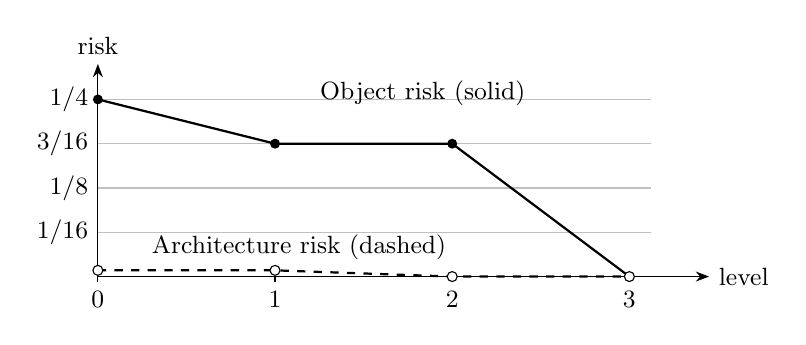
\begin{tikzpicture}[x=2.25cm,y=9cm,>=Stealth,every node/.style={font=\small}]
\draw[->] (0,0)--(3.45,0) node[right]{level};\draw[->] (0,0)--(0,0.30) node[above]{risk};
\foreach \x in {0,1,2,3}{\draw (\x,0)--(\x,-.007) node[below]{\x};}
\foreach \y/\lab in {0.0625/{1/16},0.125/{1/8},0.1875/{3/16},0.25/{1/4}}{\draw[gray!50] (0,\y)--(3.12,\y);\node[left] at (0,\y) {$\lab$};}
\draw[thick] (0,.25)--(1,.1875)--(2,.1875)--(3,0);
\foreach \x/\y in {0/.25,1/.1875,2/.1875,3/0}{\fill (\x,\y) circle[radius=1.8pt];}
\draw[thick,dashed] (0,.0087890625)--(1,.0087890625)--(2,0)--(3,0);
\foreach \x/\y in {0/.0087890625,1/.0087890625,2/0,3/0}{\draw[fill=white] (\x,\y) circle[radius=1.8pt];}
\node[anchor=west] at (1.2,.258) {Object risk (solid)};
\node[anchor=west] at (.25,.041) {Architecture risk (dashed)};
\end{tikzpicture}
\caption{Exact population risks: object risk $1/4,3/16,3/16,0$; architectural risk $9/1024,9/1024,0,0$. Meta-risk for the first frozen report is zero throughout.}
\end{figure}

The example is a finite logical model of differentiated evidence, not an observed performance benchmark. It exhibits how information about an architecture can leave object credit unchanged, how accurate object grading can leave architectural uncertainty unresolved, and how a meta-grade can be known even when the original judgment is not. The three frontiers need genuinely different kinds of evidence.
\section{Oracle limits and obstructions}
\subsection{Exact scoped grading is not universal oraclehood}
Corollary \ref{cor:spp} supplies a limiting evaluator. Exact recovery of the full vector of underlying targets $X,Y_\infty,A_\infty$ occurs precisely when each $X_j$, $Y_\infty$ and $Y_0$ has an $\F_\infty$-measurable version. Indeed $A_\infty=Y_\infty-Y_0$; if both the opportunity and its increment are recovered then so is $Y_0$. This criterion concerns a declared population and target registry. It is not a claim of omniscience or a uniform algorithm for every theorem.

In the Research Director's oracle program, oraclehood is related to attained minimization of a declared ignorance measure. SPP minimizes a particular weighted prediction risk relative to its authorized evidence. Whether that constitutes oraclehood depends on whether that risk and feasible comparison class coincide with the oracle definition being used. An evaluator that has exhausted all information allowed to it may still have irreducible risk. Conversely, possessing all grades in a narrow registry need not be sufficient to solve arbitrary logical problems. Proposition \ref{prop:regret} supplies one restricted bridge from evaluation to action, not a general oracle theorem.

\begin{proposition}[No effective general stabilization guarantee]
There is a uniformly computable family of bounded monotone finite-stage architectural grades whose limits cannot be uniformly approximated to absolute error less than $1/8$ by a total algorithm.
\end{proposition}
\begin{proof}Given a machine/input index $e$, simulate it for $k$ steps. Begin with a cost-two ordinary route; when a halting trace is found, include an optional cost-one revision shortcut. Define $y_k(e)=2^{-H_k(e)}$, with $H_k(e)$ equal to two before discovery and one after. This is a sequence of finite abstract graphs indexed by discovery stage (not the single-graph gift budget of Theorem \ref{thm:joint}). The limit is $1/4$ on nonhalting inputs and $1/2$ on halting inputs. An approximation with error strictly less than $1/8$ separates them at $3/8$, deciding halting.\end{proof}
This adaptation of the computability obstruction in \cite{professor} also fits the abstract monotone-target theorem with trivial information and discovery stage as its increasing index. It does not assert that a real sovereign can admit a halting-encoded shortcut in an arbitrary formal system. Finite graph computation, existence of a limit, computability of the limit and execution of an oracle are distinct questions.

\subsection{Oracle opacity at the joint boundary}
Let $O$ be a binary oracle-status variable. If a learning gate maintains $\Prob(O=1\mid\F_n)=1/2$ at every finite level, then L\'evy's upward theorem implies the same equality at $\F_\infty$. The minimum possible squared-error risk among $\F_\infty$-measurable reports of $O$ remains $1/4$ (and the best binary classifier has error probability $1/2$). The statement holds even if every object target in the declared ledger is recovered exactly, provided the learning-gate condition is compatible with that recovery. If those targets together determine $O$, the condition cannot hold. Therefore openness of mathematical information and opacity of self-status are distinct obligations; an oracle gate has to protect against the entire accumulated transcript, not just each isolated message. The reciprocal-training conjecture of \cite{creative} is not settled by this observation.

\section{A research program and implementation contract}
\begin{definition}[Finite SPP instance]
An SPP instance is an auditable finite controller consisting of (i) a frozen registry of judgment contracts and target IDs, (ii) an independently checked BANK and immutable report archive, (iii) authorized evidence with provenance and cutoff times, (iv) object and meta-level estimators with uncertainty records, (v) a costed candidate-revision planner, and (vi) a supervisor-gated revision interface. The interface admits no unresolved or inconsistent gift, never assumes that high predicted credit is an admission certificate, and records the actual exercise of any admitted change. The instance reports its finite depth, resource usage and unresolved obligations.
\end{definition}
The state machine must preserve unique sovereign office and the historical commitments of the applicable GBG+S specification. It must distinguish proposals, authorization, verified admission and execution. No specific meaning of an unsettled gift atom is assumed. The abstract theorems do not establish consistency of that manual. Verification remains external to the claims being verified; evaluator rank cannot grant verification authority. The architecture may be evaluated under a non-sovereign abstract contract even when no GBG+S realization has been established.

A first implementation can be entirely offline: finite graphs, exact rational Bayesian tables and a deterministic event log. Freeze test targets, training exposure, verifier, cost units, revision budget and scoring registry. Compare object-only, object-plus-meta, architecture-only and joint controllers under equal total resource budgets. Record verified settlement frequency, cost, calibration error, weighted risk, creative yield, false admission attempts and the difference between forecast and realized architectural utility. Use separate held-out tasks to guard against fitting the scoring system. Ablate redundant versus genuinely informative reviewers and include a protected unchanged baseline. Report resource costs for computing grades and for verifying architectural changes. This is an experimental specification, not a completed deployment.

\begin{conjecture}[SPP capability bridge]
The proposed research conjecture is that there exist nontrivial oracle-relevant ATP workload families, increasing finite legal policy classes and a resource schedule for which an effective, independently verified SPP protocol simultaneously achieves (i) vanishing decision-relevant estimation error on the active action sets (for example the unweighted squared-error condition of Theorem \ref{thm:growing}), (ii) vanishing optimization error, and (iii) convergence of the best accessible policy values to a separately declared oracle capability value, all without changing the evaluation contract. The intended workload family, oracle benchmark and resource schedule must be specified independently of the resulting scores before this conjectural existence claim can be tested. As stated this is a research schema, not a fully specified decision problem.
\end{conjecture}
The requirements in the conjecture distinguish coverage, calibration, optimization and admissibility. In a fixed finite action class the regret proposition gives the risk-to-decision implication. For increasing classes, one additionally needs a rate controlling errors on the active set, approximation of the capability supremum, and a legal schedule of charged operations. The existence of such schedules for the intended ATP family is the open research problem, not a consequence of martingale convergence. A useful negative result would exhibit an oracle-relevant class in which any effective SPP controller fails one of these requirements.

\section{Settlement register and conclusion}
\small
\begin{tabularx}{\textwidth}{@{}>{\raggedright\arraybackslash}p{0.46\textwidth}>{\raggedright\arraybackslash}X@{}}
\toprule
Claim & Status in this manuscript\\
\midrule
Typed logical and recursive credit ledger, exact risk decrement, exact recovery criterion & Proved under a fixed countable registry and nested authorized evidence.\\
Joint architectural and informational limit, all iterated limits & Proved for common evidence and bounded ordered targets; includes the full directed limit.\\
Joint three-index SPP limit & Proved by tail control and joint convergence.\\
Architectural forecast versus exercised gain & Defined separately; robust interval comparison proved.\\
Risk-to-decision regret bound and moving-target drift & Proved under stated action and filtration contracts.\\
General oraclehood, effective convergence rates, full GBG+S realization & Open; no claim of independent proof-kernel certification.\\
Finite experiment & Exact synthetic calculation under the specified symmetric signal channel, not an ATP performance trial.\\
\bottomrule
\end{tabularx}
\normalsize

The Sovereign Professor of Professors is best understood as a structured limit rather than a single super-grader. It preserves the question asked of logical objects, retains questions about the accuracy of those who evaluate them, and adds questions about how the underlying machinery may be lawfully improved. The central convergence theorem allows the three frontiers to meet without assuming that they are identical. The operational challenge is to approach that boundary with finite, auditable and useful decisions. The mathematical challenge is to determine when convergence of the right partial-credit coordinates yields convergence of the capabilities that actually matter.

\paragraph{Revision note (001v2).} Atlas-style review tightened the grading counterexample, registry and measurability conventions, the distinction between feasible and exercised revisions, decision-model assumptions, the finite signal model, and the scope of the capability conjecture. The main convergence results and the independent verification boundary are retained. This is a mathematical editorial audit, not external proof-kernel certification.

\begin{thebibliography}{9}
\bibitem{creative} B. Tenneson (research director), Picard (mathematical development), \emph{The Creative Sovereign: Partial Credit, Architectural Creativity, and Reciprocal Training in the 24th Century}, 001v2, 26 November 2026. \href{https://btenneson.github.io/pub/cs.LO_Logic_in_Computer_Science/the_creative_sovereign_001v2/}{Published manuscript.}
\bibitem{professor} B. Tenneson (research director), Picard--CIIP (mathematical development), \emph{The Professor of Professors: Probabilistic Partial Credit, Recursive Awareness, and the Oracle Limit}, 001v2, 26 November 2026. \href{https://btenneson.github.io/pub/cs.LO_Logic_in_Computer_Science/the_professor_of_professors_001v2/}{Published manuscript.}
\bibitem{williams} D. Williams, \emph{Probability with Martingales}, Cambridge University Press, 1991. (Conditional expectation, martingale convergence and L\'evy's upward theorem.)
\end{thebibliography}
\end{document}
